%%%%%%
%
% $Autor: Srikanth Nanda $
% $Datum: 2025-10-22 11:15:45Z $
% $Pfad: githubtemplate/Template/Presentations/RaspberryPiCameraModule2/slides/rename.tex $
% $Version: 4620 $
%
%
% !TeX encoding = utf8
% !TeX root = Rename
%
%%%%%%



\Mysection{Raspberry Pi Camera Module V2}

\STANDARD{Raspberry Pi Camera Module V2}
{
	\begin{figure}
		\centering 
		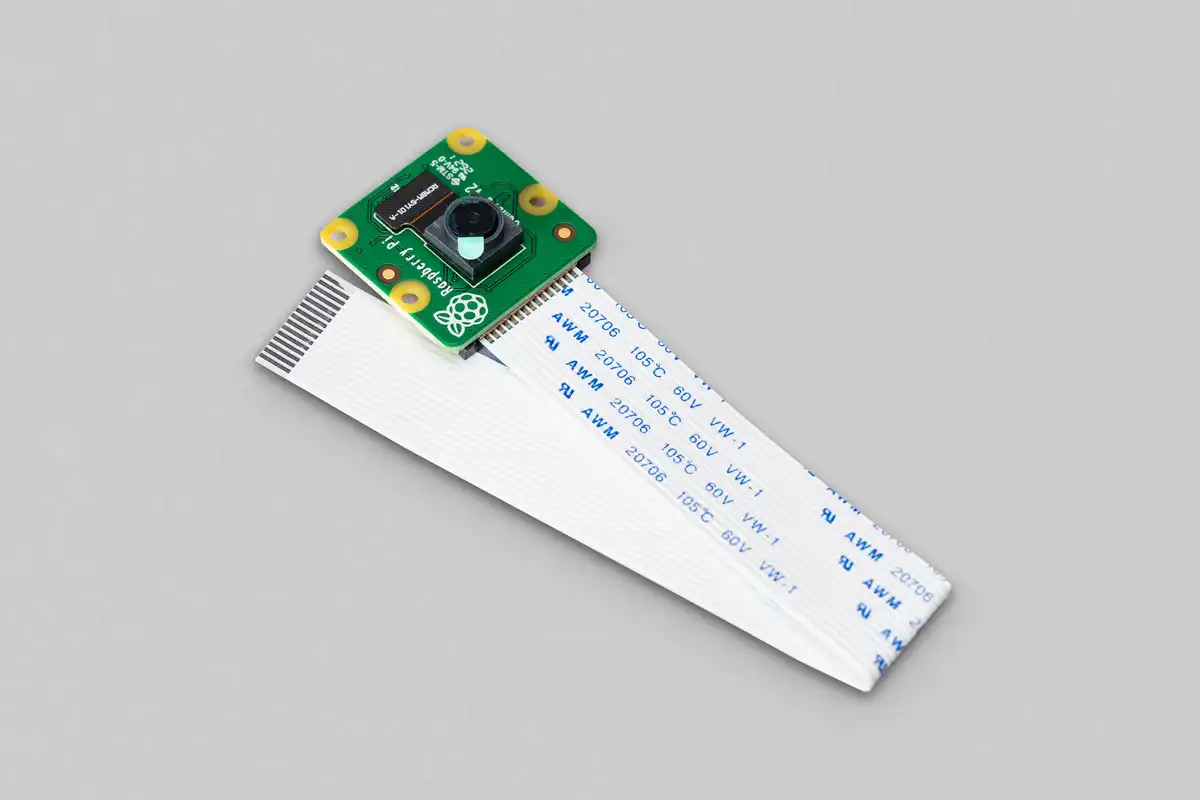
\includegraphics[width=0.5\linewidth]{../RaspberryPiCameraModule2/images/RSPV2.jpg}
		\caption{Raspberry Pi Camera Module V2}
	\end{figure}
}
\STANDARD{What is the Raspberry Pi Camera Module V2?}
{
	The \textbf{Raspberry Pi Camera Module V2} is a compact 8-megapixel camera module based on the Sony IMX219 sensor (commonly used in research and maker projects). It supports still images up to 3280x2464 and video modes up to 1080p30/720p60. \\
	\vspace{2mm}
	Key references: Pagnutti et al. (2017) for calibration/use in scientific imaging; Bowman et al. (2020) for flat-field / colour correction; Yang et al. (2023) for field-deployable Pi-based camera systems. \\
	\vspace{1mm}
	Cite examples: \cite{Pagnutti:2017, Bowman:2020, Yang:2023}
}

\Mysection{Hardware \& sensor details}
\STANDARD{Sensor and optics}
{
	\begin{itemize}
	\item Sensor: Sony IMX219 (8 MP, 1.4µm pixels) used on the \textbf{Raspberry Pi Camera Module V2}.
	\item Interface: CSI-2 ribbon connector to Raspberry Pi single-board computers.
	\item Important: stock lens and firmware shading correction are tuned for the stock optics — removing the lens or adding custom optics requires calibration and flat-field correction. \cite{Bowman:2020}
	\end{itemize}
}
\Mysection{Calibration \& image corrections}
\STANDARD{Calibration steps}
{
\textbf{Camera intrinsics \& distortion:}
	\begin{enumerate}
	\item Capture chessboard / checkerboard images using the \textbf{Raspberry Pi Camera Module V2}.
	\item Use OpenCV calibrateCamera() to compute intrinsic matrix \(K\) and distortion coefficients.
	\item Save the calibration file and use remapping/undistort at capture time to remove lens distortion.
	\end{enumerate}
\vspace{2mm}
	\textbf{Flat-field and colour corrections:} Bowman et al. provide methods to correct vignetting and colour crosstalk when using alternate optics (lens shading tables and colour unmixing). \cite{Bowman:2020, BowmanArXiv:2019}
}

\Mysection{Applications}
\STANDARD{Common and research applications}
{
	The \textbf{Raspberry Pi Camera Module V2} is widely used in:
	\begin{itemize}
	\item \textbf{Time-lapse ecology / phenology monitoring} — low-power PiCAM deployments in Arctic and remote sites. \cite{Yang:2023}
	\item \textbf{Low-cost photogrammetry / UAV experiments} — prototyping airborne imaging solutions and orthomosaic capture.
	\item \textbf{Educational vision projects and robotics} — computer vision teaching, object detection, SLAM prototyping.
	\item \textbf{Custom optics / scientific imaging} — with corrected flat-field \& colour unmixing it becomes suitable for quantitative imaging. \cite{Pagnutti:2017, Bowman:2020}
	\end{itemize}
}

\Mysection{Field deployment (example: PiCAM)}
\STANDARD{PiCAM: low-power time-lapse system}
{
The PiCAM system uses Raspberry Pi SBC + \textbf{Raspberry Pi Camera Module V2} and low-power scheduling to capture long-term time series for plant phenology monitoring in Arctic conditions — see Yang et al. (2023) for hardware design, power management, and deployment lessons. \cite{Yang:2023}
}

\Mysection{Practical tips}
\STANDARD{Tips for better scientific images}
{
	\begin{itemize}
	\item Keep the stock lens if you don't need custom optics; otherwise run flat-field correction per Bowman et al. \cite{Bowman:2020}
	\item Use RAW capture modes where possible (to avoid firmware JPEG processing) and apply your own demosaicing and corrections.
	\item Protect the module from moisture/temperature extremes when doing field work (PiCAM design discusses enclosures and power schedules). \cite{Yang:2023}
	\end{itemize}
}

\Mysection{Connecting Raspberry Pi Camera Module V2 to NVIDIA Jetson Nano}
\STANDARD{Hardware Connection \& Setup}
{
\textbf{Required components:}
\begin{itemize}
	\item NVIDIA Jetson Nano Developer Kit (2GB or 4GB).
	\item Raspberry Pi Camera Module V2 (Sony IMX219).
	\item CSI ribbon cable (15-pin).
\end{itemize}
\vspace{2mm}
\textbf{Connection steps:}
\begin{enumerate}
	\item Power off the Jetson Nano completely.
	\item Locate the CSI camera connector (near the USB ports).
	\item Gently lift the black locking tab on the connector.
	\item Insert the camera’s ribbon cable with the metal contacts \textbf{facing the HDMI port}.
	\item Push the cable in fully, then press the locking tab down.
	\item Power on the Jetson Nano.
\end{enumerate}
\vspace{2mm}
}
\STANDARD{Verification:}
{
	Use the \texttt{ls} command to check for video devices in the \texttt{/dev/} directory.
	You should see a device such as \texttt{/dev/video0}.
	
	
	
	If you are getting an error here, the issue is likely with the GStreamer plugins or your hardware setup, not the LaTeX code itself!
	
	Reference designs and sensor-level evaluation of the Raspberry Pi Camera Module V2 are provided by Pagnutti et al. \cite{Pagnutti:2017} and Bowman et al. \cite{Bowman:2020}.
}


\Mysection{Calibration and Testing Code for Raspberry Pi Camera Module V2}
\STANDARD{Camera Calibration and Testing}{
	\textbf{Purpose:} To correct geometric distortion, flat-field variation, and colour in images from the \textbf{Raspberry Pi Camera Module V2} as recommended by \cite{Pagnutti:2017, Bowman:2020}.
	
	\vspace{2mm}
	
	\textbf{1. Live Camera Testing}
	
	Before calibration, verify the camera feed using this simple live test script, \texttt{LiveCameraTest.py}.
	
	\lstinputlisting[language=Python,style=mystyle,firstline=1,firstnumber=1]{Code/LiveCameraTest.py}
	
	\vspace{2mm}
	\textbf{2. Capture Calibration Images}
	
	The script \texttt{CaptureCaliberationImages.py} uses the optimized GStreamer pipeline for the Jetson Nano to capture sequential checkerboard images.
	
	\lstinputlisting[language=Python,style=mystyle,firstline=1,firstnumber=1]{Code/CaptureCaliberationImages.py}
	
	\vspace{2mm}
	\textbf{3. OpenCV Calibration Code}
	
	The distortion and flat-field calibration steps correspond to the approaches demonstrated in \cite{Bowman:2020}, while spectral and radiometric performance metrics follow \cite{Pagnutti:2017}. The following script, \texttt{CameraCalibration.py}, performs the actual computation.
	
	\lstinputlisting[language=Python,style=mystyle,firstline=1,firstnumber=1]{Code/CameraCalibration.py}
}
	
	
	\Mysection{Applications of Raspberry Pi Camera Module V2}
	\STANDARD{Example Research and Engineering Uses}{
	The \textbf{Raspberry Pi Camera Module V2} is a low-cost, flexible imaging device used in numerous domains:
	
	\vspace{2mm}
	\textbf{Environmental and ecological monitoring}
	\begin{itemize}
		\item The PiCAM system deploys the camera for long-term monitoring of plant phenology in Arctic ecosystems. \cite{Yang:2023}
		\item Combines low power scheduling, time-lapse imaging, and weatherproof housings.
	\end{itemize}
	
	\vspace{2mm}
	\textbf{Scientific imaging and calibration research}
	\begin{itemize}
		\item Pagnutti et al. \cite{Pagnutti:2017} demonstrate how to calibrate the sensor for scientific imaging, measuring radiometric linearity, spectral response, and noise.
		\item Bowman et al. \cite{Bowman:2020} present correction models for lens shading and colour mixing that make the module suitable for quantitative microscopy and optical experiments.
	\end{itemize}
	
	\vspace{2mm}
	\textbf{Robotics and computer vision}
	\begin{itemize}
		\item Used for object detection, visual odometry, and SLAM on Jetson Nano and Raspberry Pi.
		\item Integration with TensorRT or PyTorch allows real-time inference on embedded systems.
	\end{itemize}
	
	\vspace{2mm}
	\textbf{UAV and remote sensing platforms}
	\begin{itemize}
		\item Mounted on drones for lightweight orthomosaic mapping and photogrammetry; see performance evaluations in \cite{Pagnutti:2017}.
	\end{itemize}
	
	\vspace{2mm}
	\textbf{Summary:}
	\begin{itemize}
		\item Low cost and open software support make the \textbf{Raspberry Pi Camera Module V2} ideal for education, research, and embedded systems.
		\item Calibration and colour correction (Bowman et al. 2020) and low-power design (Yang et al. 2023) enable scientific-grade imaging on a budget.
	\end{itemize}
}

	